\documentclass[12pt]{beamer}

\usepackage{ucs}
\usepackage[utf8x]{inputenc}

\usepackage[australian]{babel}
\usepackage[T1]{fontenc}
\usepackage{graphicx}

\usetheme{Berkeley}

\title{PODD Ontology Driven Database}
\author{Dr Peter Ansell}
\institute{University of Queensland}
\date{13 March 2012}

\begin{document}

\begin{frame}
\titlepage
\end{frame}


\begin{frame}
\frametitle{Background} 

\begin{itemize}
 \item PODD was designed by Yuan-Fang Li and Gavin Kennedy for the High Resolution Plant Phenomics Centre
 \item Implemented between 2009 and 2011
\end{itemize}

\end{frame}

\begin{frame}
\frametitle{Motivation} 

\begin{itemize}
 \item Flexible scientific experiment management
 \item Use RDF and OWL technology to support science
\end{itemize}


\end{frame}

\begin{frame}
\frametitle{Example} 

Simultaneous Phenotyping of Drought Stress Tolerance in Arabidopsis OST1-2 Mutant and Wild Type 

\vskip 12pt


Credit to Xueqin Wang for the example design : \url{http://podd.plantphenomics.org.au/podd/object/poddObject:838}

\end{frame}

% PODD Design/Architecture as a blank slide
\bgroup
\usebackgroundtemplate{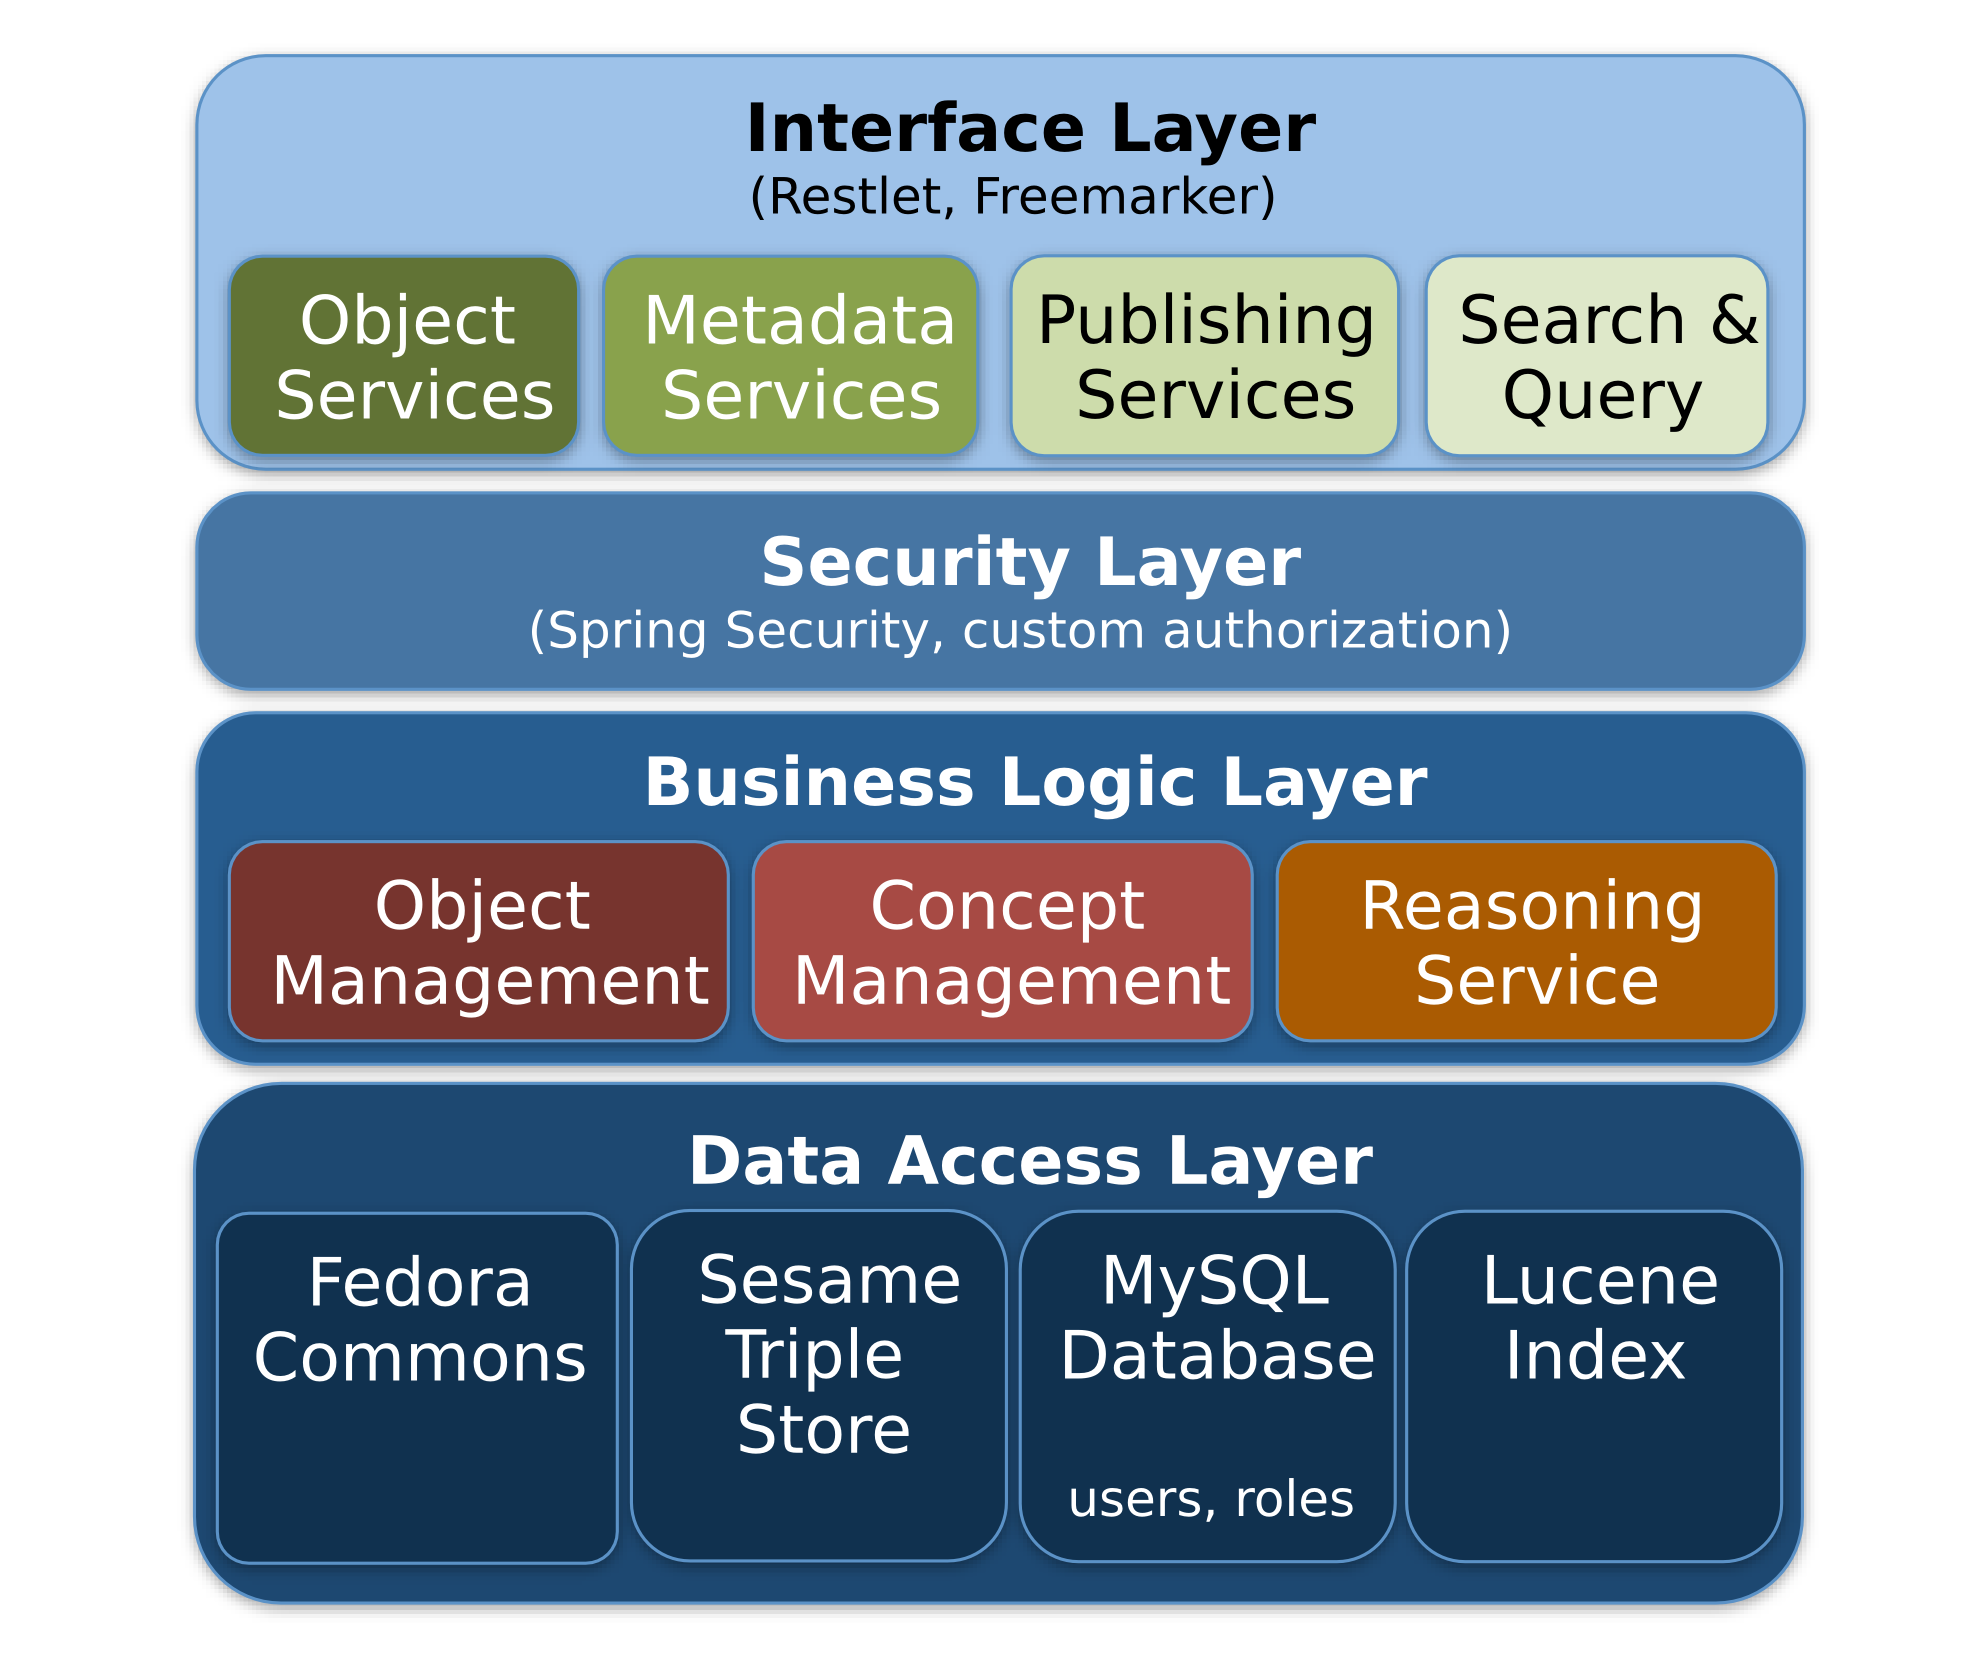
\includegraphics[
width=\paperwidth,
height=\paperheight,
keepaspectratio=true
]{podd_arch.png}}
\begin{frame}[plain]{}
\end{frame}
\egroup


% PODD Phenomics Ontology as a blank slide
\bgroup
\usebackgroundtemplate{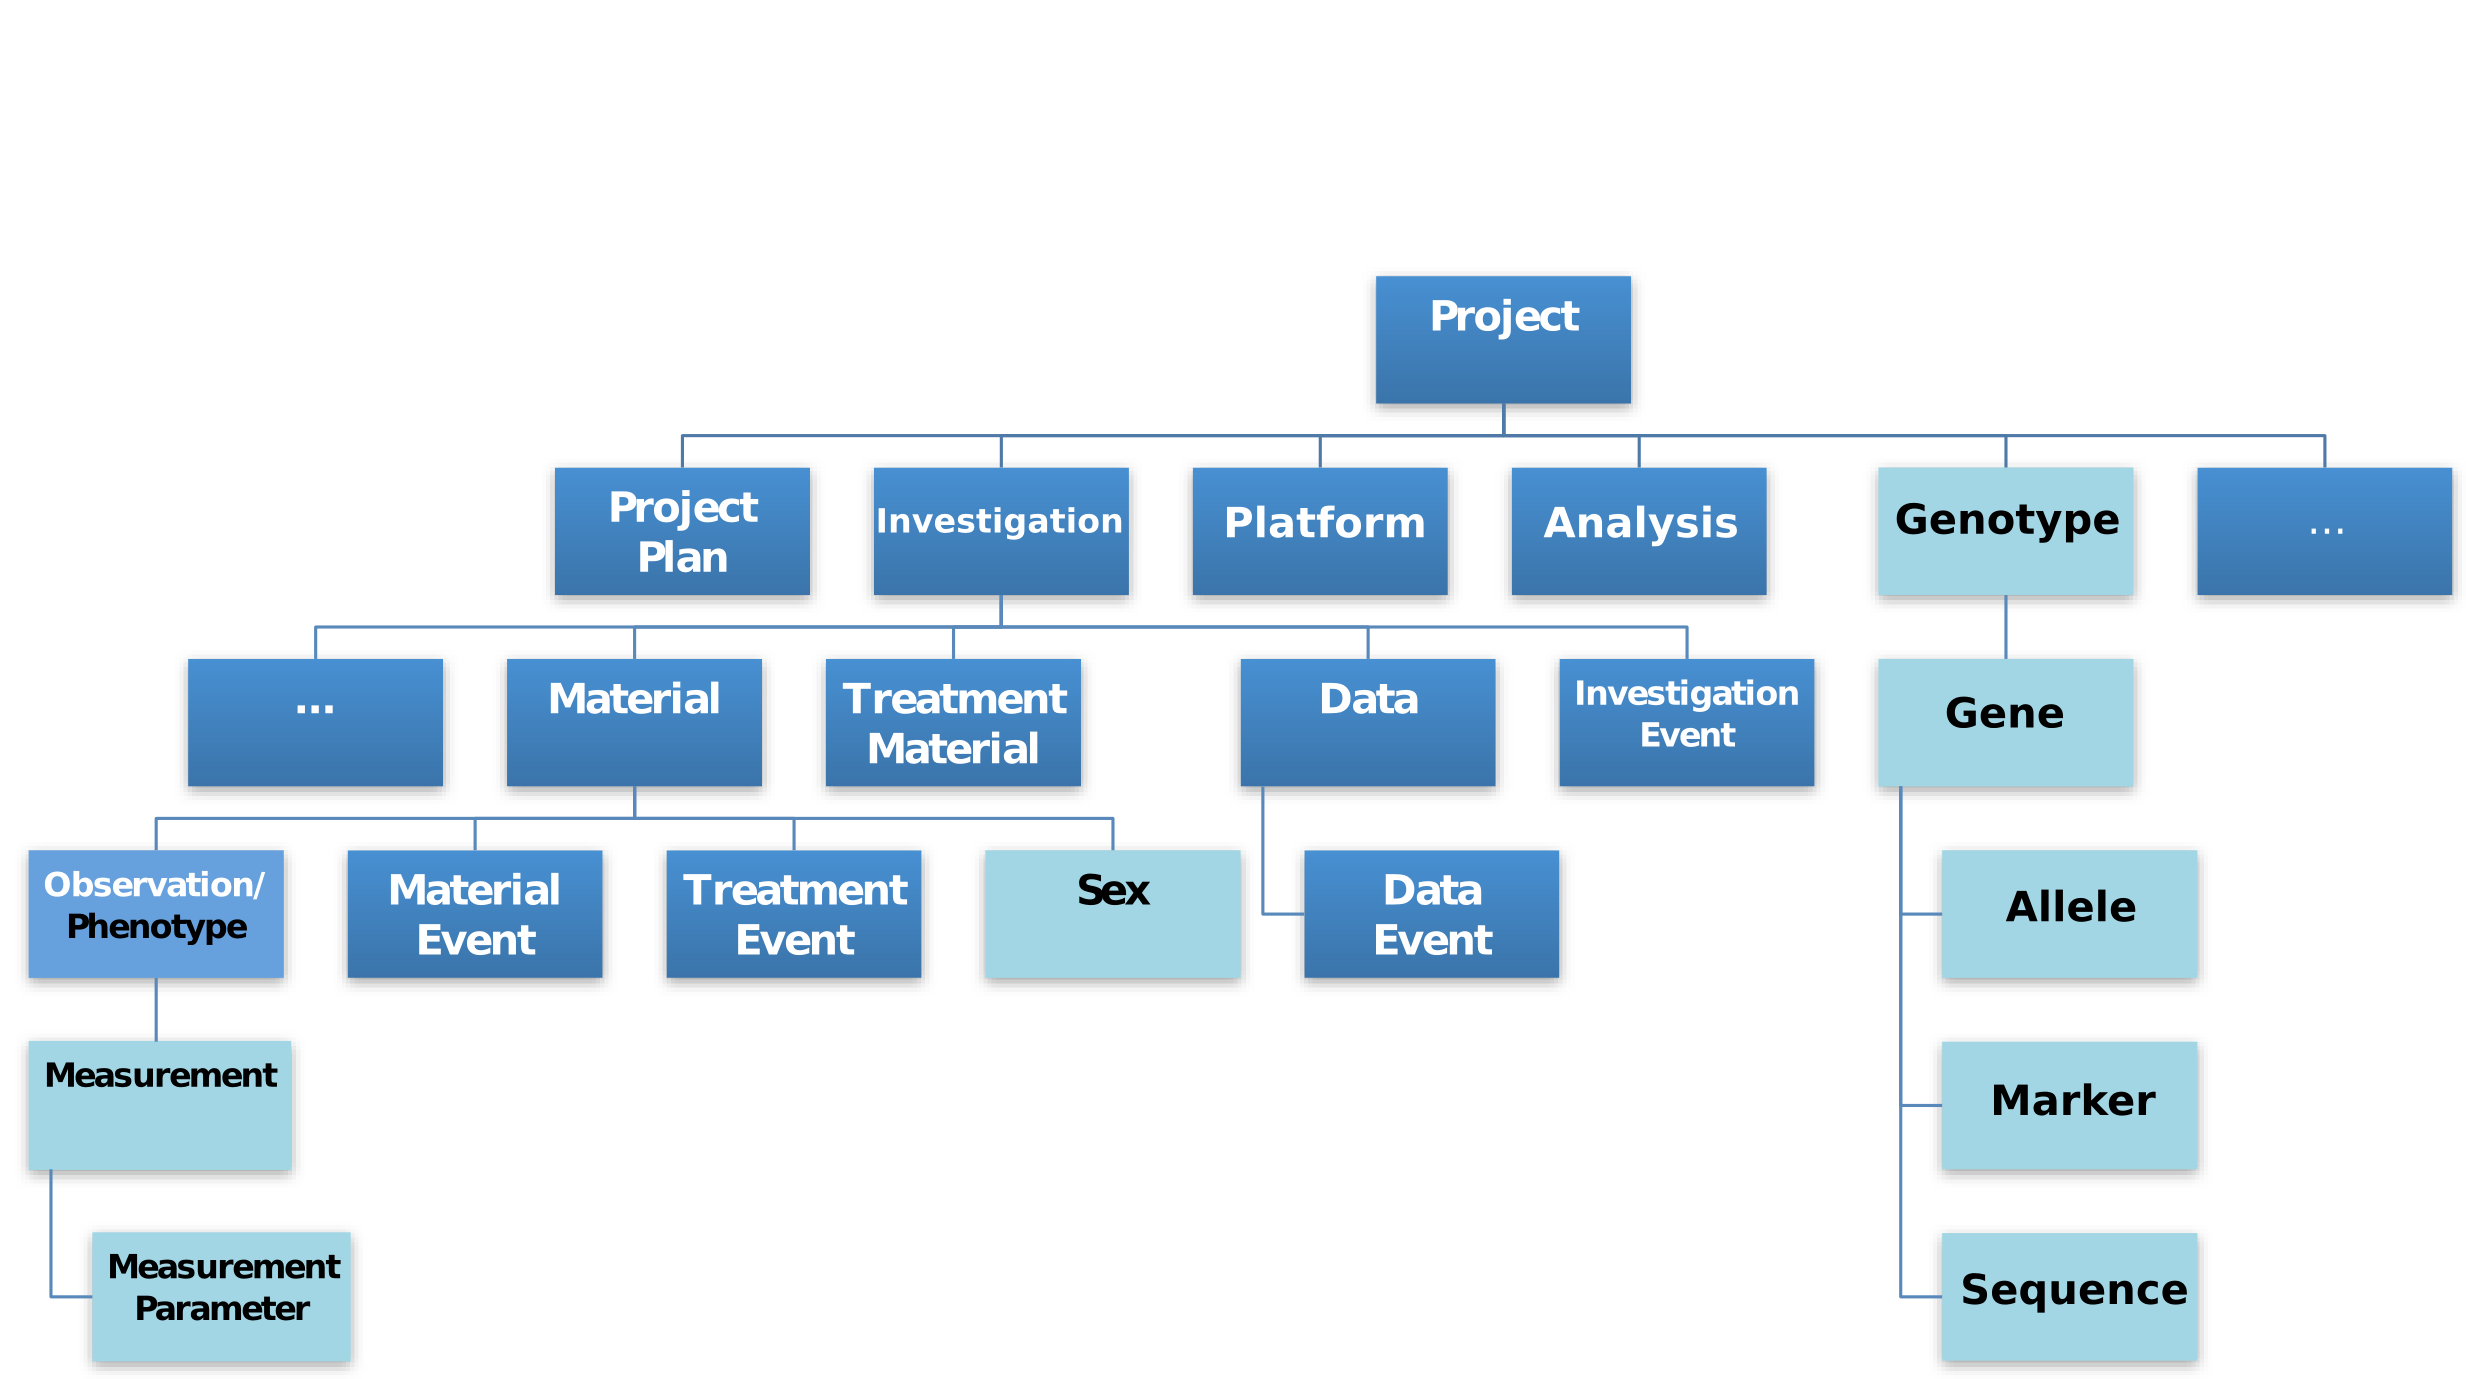
\includegraphics[
width=\paperwidth,
height=\paperheight,
keepaspectratio=true
]{podd_ont.png}}
\begin{frame}[plain]{}
\end{frame}
\egroup

\begin{frame}
\frametitle{Demo} 

\url{http://podd.plantphenomics.org.au/podd}

\end{frame}

\begin{frame}
\frametitle{Evaluation}

Pros:

\begin{enumerate}
 \item Flexible : Simultaneously supports different experiments
 \item Adaptable : Supports additions and changes to schema ontologies
\end{enumerate}

Cons:

\begin{enumerate}
 \item Current implementation does not scale with experiment size
 \item Only supports OWL-1.1
 \item Uses old versions of Fedora and Spring
\end{enumerate}


\end{frame}

\begin{frame}
\frametitle{Next steps}

\begin{itemize}
 \item Use upcoming SPARQL 1.1 Query and Update standards
 \item Support OWL-2
 \item Pure SPARQL access using a single database
 \item Support links from experiments to other RDF documents
\end{itemize}


\end{frame}


\begin{frame}
\frametitle{Questions}

\begin{center}
Open source code can be found online at:

\url{https://github.com/podd}

\vskip 12pt

My email is: peter.ansell@uq.edu.au
\end{center}
\end{frame}

\end{document}


